\documentclass[12pt]{article}
\usepackage{amssymb,graphicx}

\pagestyle{empty}
%\textwidth 6.5in
%\textheight 10in
%\topmargin -20mm
%\parskip 1ex
%\input epsf

\newcommand{\vb}{\bf}

\begin{document}

\begin{center}
\bf{Worksheet 1 --- Math 126 --- Summer 2010}
\end{center}
\bigskip
This worksheet should help with your geometric visualization and
understanding, which will help you with other problems in this
chapter.  Also, there may be quiz or test problems which are similar
some of these questions.

\begin{enumerate}
\item Suppose that $\vb{a}$ and $\vb{b}$ are nonzero vectors.
 \begin{enumerate}
        \item Show by examples that comp$_{\vb{a}}\vb{b}$
                                and  comp$_{\vb{b}}\vb{a}$
        can be the same and can be different.
        What conditions on  $\vb{a}$ and $\vb{b}$ will
                guarantee they are the same?
        \item Your friend who skips class frequently says, ``I'm confused.
        Isn't $\vb{a} \cdot \vb{b} = \vb{b} \cdot \vb{a}$?
        If that is true, how can  comp$_{\vb{a}}\vb{b}$
                                and  comp$_{\vb{b}}\vb{a}$
        be different?''  What is your answer?
        \item Show by examples that proj$_{\vb{a}}\vb{b}$
                                and  proj$_{\vb{b}}\vb{a}$
        can be the same and can be different.
        What conditions on   $\vb{a}$ and $\vb{b}$ will
                guarantee they are the same?
 \end{enumerate}

\item Decide for each expression below whether it is a vector (\textbf{V}),
a scalar (\textbf{S}), or nonsense (\textbf{N}).
Note that $\vb{a}, \vb{b}, \vb{u}$, and $\vb{v}$ are vectors, while
$c$ and $d$ are scalars.

\hfill                                  Circle one: \hspace*{.2in}
 \begin{enumerate}
        \item ${\vb a} \cdot ({\vb u} - c{\vb v})$
                \hfill \textbf{V} \qquad \textbf{S} \qquad \textbf{N}
        \medskip
        \item ${\vb a} \cdot ({\vb b} + c)$
                \hfill \textbf{V} \qquad \textbf{S} \qquad \textbf{N}
        \medskip
        \item $(c + d) \cdot {\vb a}$
                \hfill \textbf{V} \qquad \textbf{S} \qquad \textbf{N}
        \medskip
        \item ${\vb u} {\vb v}$
                \hfill \textbf{V} \qquad \textbf{S} \qquad \textbf{N}
        \medskip
        \item $\displaystyle{\frac{{\vb a}}{c}}$
                \hfill \textbf{V} \qquad \textbf{S} \qquad \textbf{N}
        \medskip
        \item $\displaystyle{\frac{c}{{\vb a}}}$
                \hfill \textbf{V} \qquad \textbf{S} \qquad \textbf{N}
 \end{enumerate}
\vfill\eject
\item Determine whether each of the following statements is true or false. If it is true, prove it.
If it is false (that is, doesn't
hold for every case), give a counterexample.  Note that ${\vb a}$ and
${\vb b}$ are vectors and $c$ is a scalar.
   \begin{enumerate}
        \item If ${\vb a} \cdot {\vb b} = {\vb 0}$, then at least one of
                ${\vb a}$ or ${\vb b}$ must be the zero vector.
        \item If $c{\vb a} = {\vb 0}$, then
                either $c = 0$ or  ${\vb a} = {\vb 0}$.
   \end{enumerate}

\bigskip
\bigskip
Here are two three-dimensional coordinate grids for drawing the graphs
in problems 4 and 5.

\bigskip

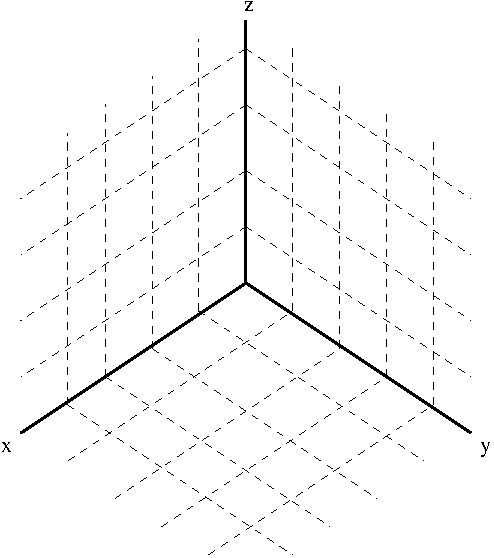
\includegraphics[width=2.1in]{3Dgrid2} \hfil
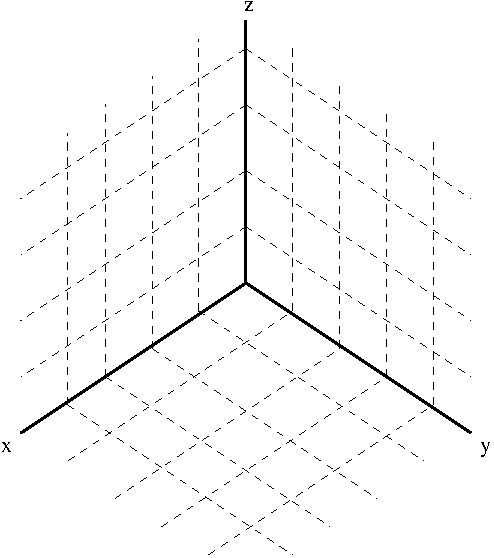
\includegraphics[width=2.1in]{3Dgrid2}

\bigskip

 
\item 
Find the equation and sketch the graph of a plane that is 
parallel to the $yz$-coordinate plane and contains the point $(2,1,3)$.
How is this plane related to the other two coordinate planes,
the $xy$-coordiante plane and the $xz$-coordinate plane?\\

\item 
Graph the plane $P$ given by the equation  $x+z=2$.\\
Is $P$ parallel to any of the coordinate planes?\\
Is $P$ perpendicular to any of the coordinate planes?\\
Is $P$ parallel to any of the coordinate axes?\\
Is $P$ perpendicular to any of the coordinate axes?\\
What fact about the equation for $P$ immediately gives you the anwer to all
of these questions?
\vfill\eject
\item Decide by yourself whether each of the following is true or false. 
Compare answers with one or two neighbors, then
confirm your answers by using pieces of paper and/or a desktop
as models for planes, and pens and/or pencils as models for lines. 
\begin{enumerate} 
 \item Two lines perpendicular to the same plane are parallel.
 \item Two lines parallel to the same plane are parallel.
 \item Two planes perpendicular to the same (third) plane are parallel.
 \item Two planes parallel to the same (third) plane are parallel.
 \item Two lines perpendicular to the same (third) line are parallel
 \item Two lines parallel to the same (third) line are parallel.
 \item Two planes either intersect or are parallel
 \item Two planes perpendicular to the same line are parallel.
 \item Two planes parallel to the same line are parallel.
 \end{enumerate}

\end{enumerate}

\end{document}
